\documentclass{article}
\usepackage[T1]{fontenc}

\usepackage{graphicx}
\usepackage{listings}
\begin{document}

\title{FOSS Lab Report}
\author{Gokul K\\[2\baselineskip]
Roll Number: 21\\[2\baselineskip]}
\date{02 February 2020}

\maketitle

\setcounter{section}{9}
\section{Shell Programming VI}
\subsection{Aim}
Write a shell script that displays a special listing showing the
permissions, size filename and last modification time of filename
supplied as arguments. Provide suitable headers using the printf
command.


\subsection{Source Code}
\begin{verbatim}
    #! /bin/bash

    # Gokul K
    # Roll No: 21
    # 25-01-2020

    # Write a shell script that displays a special listing showing the
    # permissions, size filename and last modification time of filename
    # supplied as arguments. Provide suitable headers using the printf
    # command.
    
    if [[ $# -ne 1 ]]
    then
        echo "Invalid number of arguments"
        exit
    fi
    
    if [[ ! (-f $1) ]]
    then
        echo "$1 not a file"
        exit
    fi
    
    perm="`stat -c %A $1`"
    size="`stat -c %s $1`"
    fname="`stat -c %n $1`"
    modtime="`stat -c %y $1`"
    
    printf "Permissions: %s\nSize: %dB\nName: %s\nLast Modified:\
    %s %s %s\n" $perm $size $fname $modtime
\end{verbatim}

\subsection{Program Description}
stat is a command used to display details of a file. \%A flag displays the 
permission, \%s displays the size, \%n displays the filename and \%y displays
the modification time of a file

\subsection{Output}
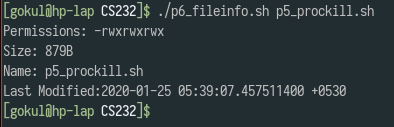
\includegraphics[width=0.9\textwidth]{img/p10.png}\newline

\subsection{Result}
The above program is run on Manjaro Linux shell. The details of the file
were obtained as result.
\end{document}